\documentclass{beamer}

\usetheme{Padova}

\title{Uso di un modello BERT per la correzione di errori generati dal processo di OCR su dati testuali}
\subtitle{Tesi di Laurea Magistrale in Informatica}
\author{Sebastiano Caccaro}
\date{17 Dicembre 2021}
\usepackage[italian]{babel} 
\usepackage{color, colortbl}
\usepackage{array}
\usepackage{pdfpages}
\usepackage{anyfontsize}
\usepackage{adjustbox}





\definecolor{grigioS}{HTML}{484F59}
\definecolor{grigioC}{HTML}{EDEDEF}

\usepackage{nameref}
\makeatletter
\newcommand*{\currentname}{\@currentlabelname}
\makeatother

\AtBeginSection[]
{
    \begin{frame}
        \frametitle{\currentname}
        \tableofcontents[currentsection]
    \end{frame}
}
\newcommand{\E}{È}

\begin{document}

	\maketitle

%	\begin{frame}{Struttura}
%		\tableofcontents
%	\end{frame}

\begin{frame}
\frametitle{Indice}
\tableofcontents
\end{frame}


%%%%%%%%%%%%%%%%%%%%%%%%%%%%%%%%%%%%%%%%%%%%%%%%%%%%%%%%%%%%%%%%
\section{Introduzione}

\begin{frame}{OCR}

		L'\textbf{Optical Character Recognition}, o \textbf{OCR}, è una tecnologia tramite la quale è possibile estrarre e digitalizzare il testo presente in un'immagine.

	\begin{figure}[H]
	\centering
	{
	\begin{minipage}{0.4\textwidth}
	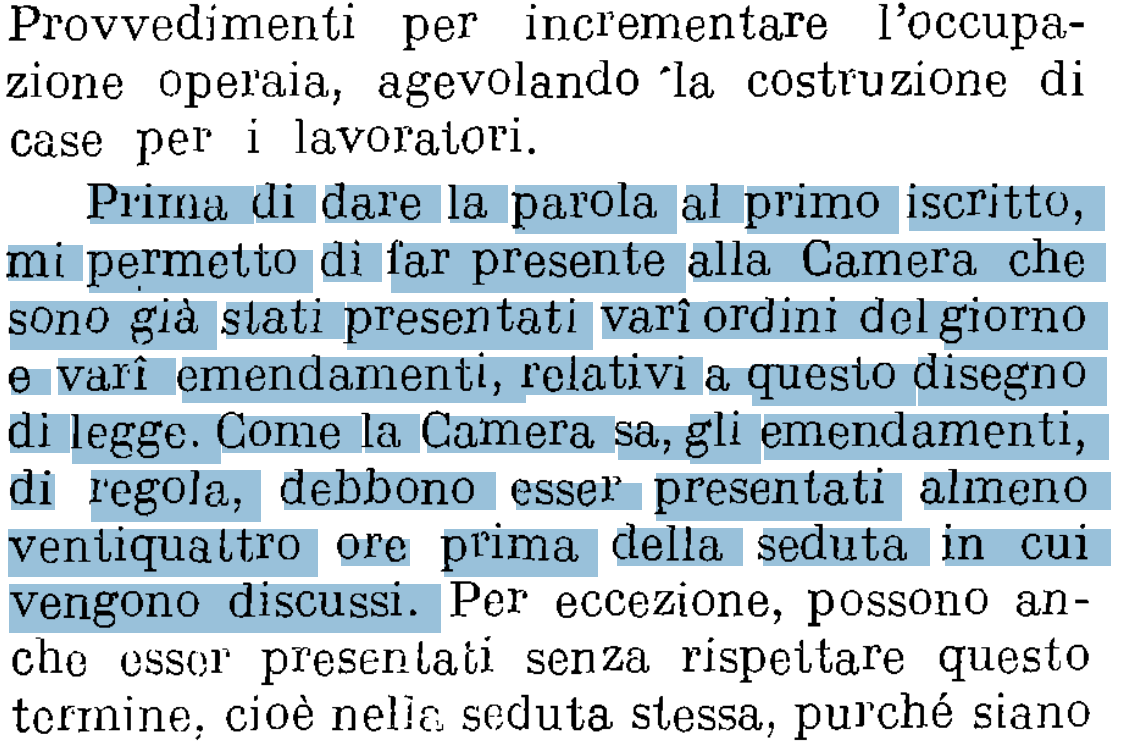
\includegraphics[width=\textwidth]{images/slides/ocr_ex.png}
	\end{minipage} \hfill
	\begin{minipage}{0.06\textwidth}
	\Large$\rightarrow$
	\end{minipage}
	\begin{minipage}{0.51\textwidth}
	\fontsize{7.7}{6}\selectfont	
	Prima. di dare la parola al primo iscritto, \\
	mi permetto di far presente alla Camera che \\
	sono già stati presentati vari ordini del giorno \\
	e var.1 emendamenti, relativi a questo disegno \\
	di legge. Come la Camera sa, gli emendamenti, \\
	di regola, debbono esser presentati alrneno \\
	ventiquattro ore prima della seduta in cui \\
	vengono discussi.
	\end{minipage}
	}
	\end{figure}
\end{frame}
	
\begin{frame}{OCR - Errori}
	L'acquisizione di testo tramite OCR può introdurre degli errori.
	\begin{table}
	\begin{tabular}{ccc}
	\adjustbox{valign=c} {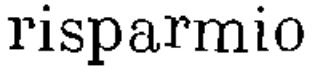
\includegraphics[height=.5cm]{images/slides/risparmio}} &
	$ \rightarrow $ & risparniio \\
	\adjustbox{valign=c} {
\includegraphics[height=.5cm]{images/slides/molto}} &
	$ \rightarrow $ & n o l l o \\
	\adjustbox{valign=c} {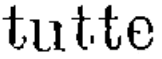
\includegraphics[height=.5cm]{images/slides/tutte}} &
	$ \rightarrow $ & t.ut.te \\
	\adjustbox{valign=c} {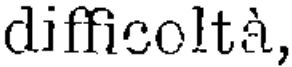
\includegraphics[height=.5cm]{images/slides/difficolta}} &
	$ \rightarrow $ & clifEir,o!t?t, \\
	\end{tabular}
	\end{table}	
	
Gli errori presenti nel testo rendono vari task di NLP meno efficaci.
\newline \newline
\E\ possibile usare tecniche di \textbf{OCR Post Processing} per correggere gli errori nel testo.
	
	
\end{frame}
%###########################################################################
\section{Stato dell'Arte}
\begin{frame}{Tipi di OCR Post Processing}
	
In letteratura sono presenti più tipi di approcci al problema dell'OCR Post Processing:
\begin{itemize}
\item n-grams: approcci statistici
\item Neural Machine Translation: correzione affrontata come una traduzione
\item \textbf{BERT}: tecnica relativamente nuova, non molti approcci in letteratura.

\end{itemize}
	
\end{frame}

\begin{frame}{BERT}
	
\textbf{BERT (Bidirectional Encoder Representation from Transformers)} è un'architettura per la costruzione di modelli linguistici sviluppata da Google sulla base dei modelli transformers.
\newline \newline
I modelli BERT sono \textbf{pre-allenati} minimizzando la perdita combinata per i task di \textbf{Masked Language Modelling (MLM)} e Next Sentence Prediction (NSP).
	
\end{frame}

%%%%%%%%%%%%%%%%%%%%%%%%%%%%%%%%%%%%%%%%%%%%%%%%%%%%%%%%%%%%%%%%%
\section{Dataset e Perturbazione}

\begin{frame}{Dataset}
\E\ necessario avere un dataset composto da \textbf{frasi parallele} per la valutazione, ma non è facile da ottenere:
\begin{itemize}
\item Correzione manuale
\item Lingua italiana
\end{itemize}\ 
\newline \newline
L'approccio scelto introduce artificialmente errori in frasi pulite.\\ \E\ detto \textbf{perturbazione}.
\end{frame}

\begin{frame}{Perturbazione}
Creazione di un sistema modulare per introdurre nel testo diversi tipi di errori:
\begin{itemize}
\item Word Error (es. risparniio, alrneno) 
\item Word Segmentation Error (es. n o l l o, t.ut.te)
\end{itemize}\
\newline
Tre diverse categorie di perturbazione, con tre livelli di intensità ciascuna:
\begin{itemize}
\item Token: \texttt{T1,T2,T3}
\item Segmentation: \texttt{S1,S2,S3}
\item Mixed: \texttt{M1,M2,M3}

\end{itemize}
\end{frame}

%%%%%%%%%%%%%%%%%%%%%%%%%%%%%%%%%%%%%%%%%%%%%%%%%%%%%%%%%%%%%%%%
\section{Metodologia}

\begin{frame}{Sistema di correzione}
Sviluppo di un sistema modulare per la correzione:
\begin{itemize}
\item Ogni modulo individua corregge una categoria di errori
\item Moduli ripetibili 
\end{itemize}

\begin{figure}[H]
\centering
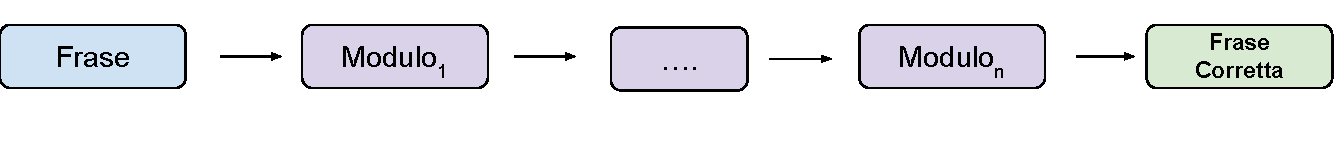
\includegraphics[width=\textwidth]{images/slides/generale}
\caption{Schema riassuntivo della pipeline di correzione}
\label{fig:met_generale}
\end{figure}


\end{frame}

\begin{frame}{Modulo di correzione Token - 1/2}
	\begin{figure}[H]	
	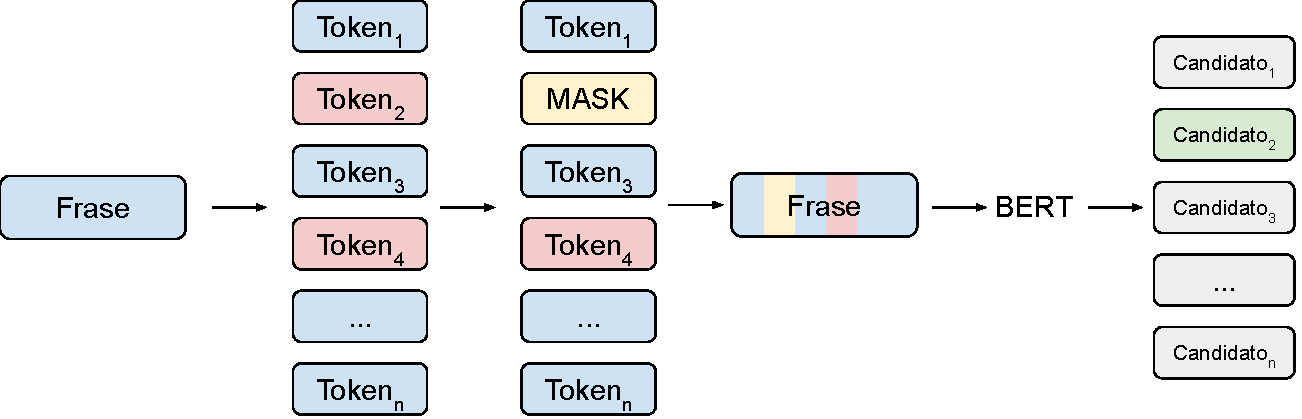
\includegraphics[width=\textwidth]{images/slides/Schema_modulo}
	\caption{Schema della prima parte del modulo di correzione Token}
	\end{figure}
\end{frame}

\begin{frame}{Modulo di correzione Token - 2/2}
	\begin{figure}[H]	
	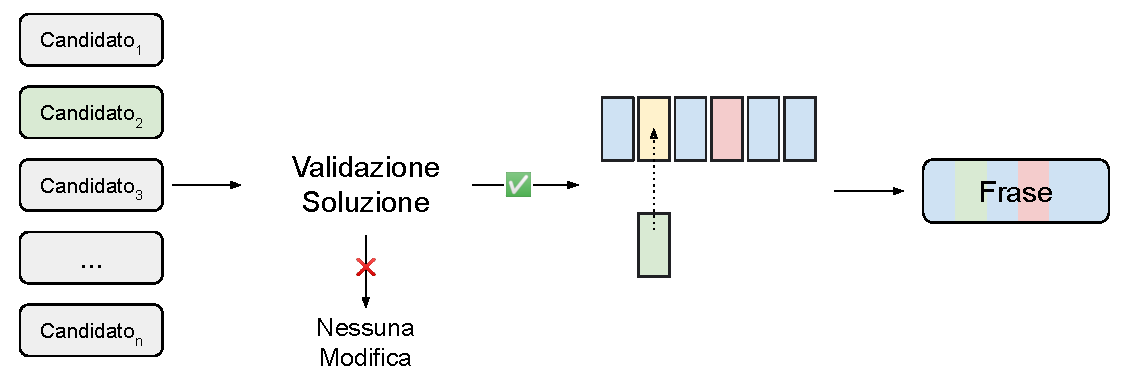
\includegraphics[width=\textwidth]{images/slides/Scelta_candidati}
	\caption{Schema della seconda parte del modulo di correzione Token}
	\end{figure}
\end{frame}

\begin{frame}{Esempio - 1/2}

\begin{center}
\textit{"che assistono ragazze in difficoltà, le persone {\color{rossoPantano} soie} e abbandonate, gli ammalati e gli anziani."}\\
$\downarrow$\\
\textit{"che assistono ragazze in difficoltà, le persone {\color{rossoPantano}[MASK]}  e abbandonate, gli ammalati e gli anziani."}\\
$\downarrow$\\
\begin{tabular}{c|ccccc}
\textbf{Token} & \textit{sole} & \textit{anziane} & \textit{povere} & \textit{care} & \textit{disabili}\\
\textbf{Prob.} & 0.42 & 0.28 & 0.08 & 0.03 & 0.01 \\
\end{tabular}
\end{center}
\end{frame}

\begin{frame}{Esempio - 2/2}
\begin{center}

\begin{tabular}{c|ccccc}
\textbf{Token} & \color{rossoPantano} \textit{sole} & \textit{anziane} & \textit{povere} & \textit{care} & \textit{disabili}\\
\textbf{Lev.Dist.} & \color{rossoPantano} 1 & 5 & 4 & 3 & 6 \\
\end{tabular}\ \\
$\downarrow$\\
\textit{"che assistono ragazze in difficoltà, le persone {\color{rossoPantano}sole}  e abbandonate, gli ammalati e gli anziani."}\\

\end{center}
\end{frame}



\section{Test e Risultati}
\begin{frame}{Metodologia di test}
\E\ stata definita una precisa metodologia di test:
\begin{itemize}
\item Test eseguiti su frasi di lunghezza differente
\item Comparazione con un altro metodo di OCR
\end{itemize}\ \\ \
\\
Cinque metriche diverse diverse, per misurare:
\begin{itemize}
\item Quantità di errori corretti
\item Quantità di errori introdotti
\end{itemize}

\end{frame}

\begin{frame}{Risultati - 1/5}
\begin{figure}[H]
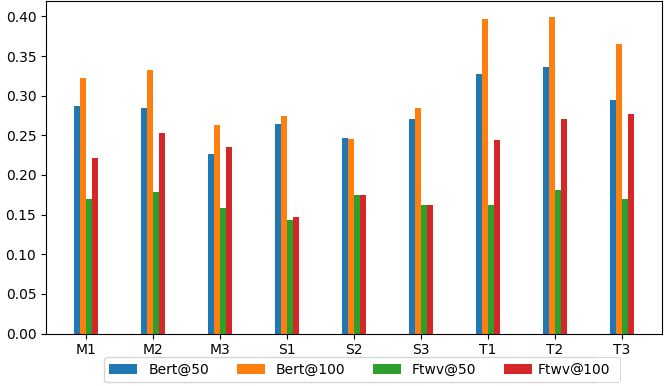
\includegraphics[width=.9\textwidth]{images/test/cp}
\caption{Errori corretti per errore presente (valori più alti = risultati migliori)}
\end{figure}
\end{frame}

\begin{frame}{Risultati - 2/5}
\begin{figure}[H]
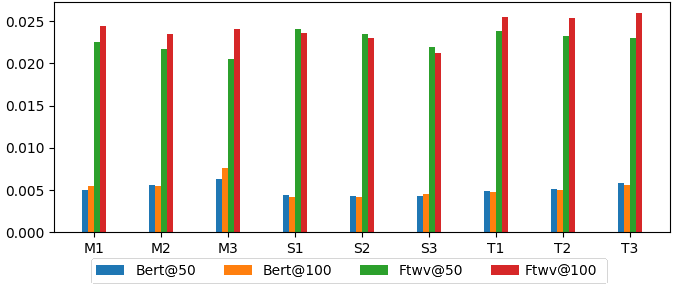
\includegraphics[width=\textwidth]{images/test/if}
\caption{Errori introdotti per carattere (valori più bassi = risultati migliori)}
\end{figure}
\end{frame}

\begin{frame}{Risultati - 3/5}
\begin{figure}[H]
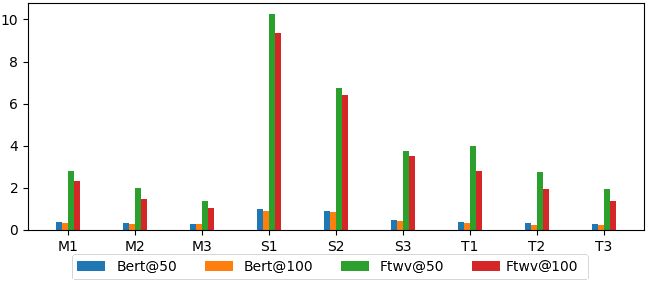
\includegraphics[width=\textwidth]{images/test/ic}
\caption{Errori introdotti per errore corretto (valori più alti = risultati migliori)}
\end{figure}
\end{frame}

\begin{frame}{Risultati - 4/5}
\begin{figure}[H]
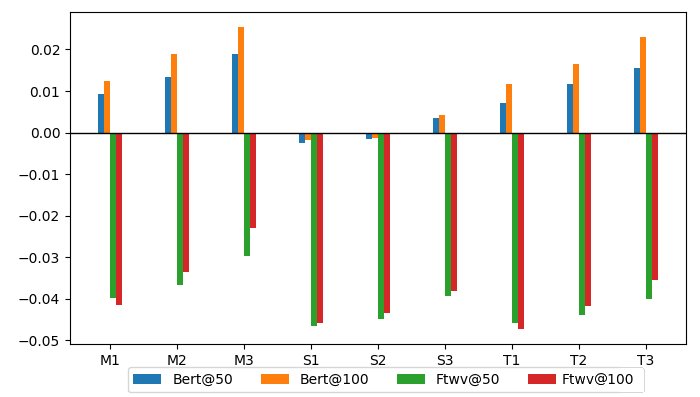
\includegraphics[width=.9\textwidth]{images/test/ldr}
\caption{Riduzione nella distanza di Levenshtein (valori più alti = risultati migliori)}
\end{figure}
\end{frame}

\begin{frame}{Risultati - 5/5}
\begin{figure}[H]
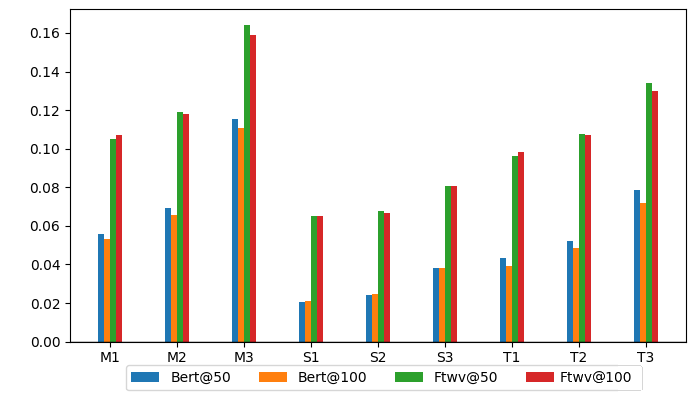
\includegraphics[width=\textwidth]{images/test/ldt}
\caption{Distanza di Levenshtein totale valori più bassi = risultati migliori)}
\end{figure}
\end{frame}

\section{Analisi dell'errore}
\begin{frame}{Analisi dell'errore}
Analisi delle di correzione del modulo di correzione Token:
\begin{itemize}
\item Senza error detection
\item Capire quali fasi sono migliorabili
\end{itemize}
\end{frame}

\begin{frame}{Risultati 1/2}
\begin{figure}[H]
\centering
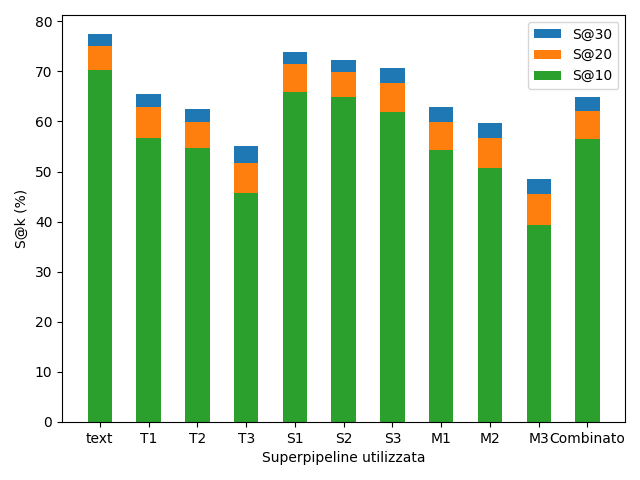
\includegraphics[width=.7\textwidth]{images/slides/overview}
\caption{Percentuale dei casi in cui BERT produce la soluzione}
\end{figure}
\end{frame}

\begin{frame}{Risultati 2/2}
\begin{figure}[H]
\centering
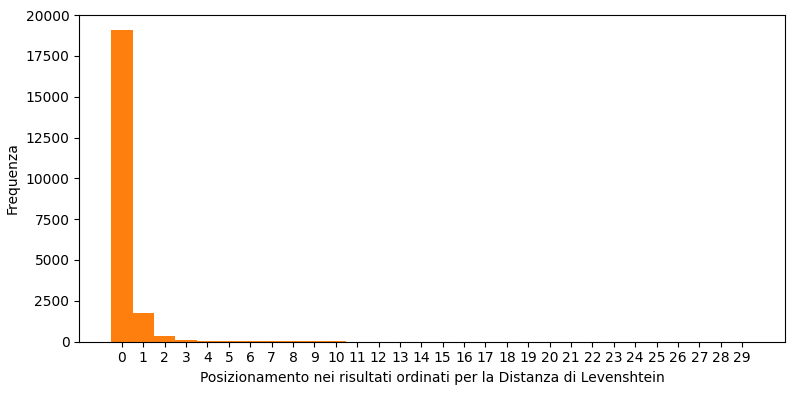
\includegraphics[width=\textwidth]{images/slides/lev_pos_Combinato}
\caption{Distribuzione della posizione della soluzione all'interno dei risultati ordinati per la distanza di Levenshtein}
\end{figure}
\end{frame}

\section{Conclusioni}
\begin{frame}{Conclusioni}
I risultati sperimentali dimostrano che:
\begin{itemize}
	\item Usare \textbf{BERT} è una via percorribile per l'OCR Post Processing
	\item A seconda del rumore presente nel testo, il sistema sviluppato corregge fra il 25\% e il 40\% degli errori corretti
	\item Rispetto agli errori corretti, il sistema sviluppato introduce un numero molto basso di nuovi errori
\end{itemize}
\end{frame}

\begin{frame}{Sviluppi futuri}
I risultati sperimentali dimostrano come il sistema di correzione abbia ampli margini di miglioramento:
\begin{itemize}
\item Applicare soluzioni più complesse per error detection e word segmentation error
\item Usare un approccio a sliding window per massimizzare la lunghezza delle frasi
\end{itemize}

\end{frame}



\begin{frame}{\ }
\huge
{Grazie per l'attenzione}
\end{frame}
	

\end{document}
